\documentclass{article}

%package setup
\usepackage{graphicx}
\usepackage{amsmath}
\usepackage{fancyhdr}
\usepackage[margin=1in]{geometry}
\usepackage{comment}
\usepackage{placeins}
\usepackage{parskip}
\usepackage{subcaption}
\usepackage{appendix}
\usepackage{soul}
\usepackage{comment}
\PassOptionsToPackage{hyphens}{url}\usepackage[hidelinks]{hyperref}
\usepackage{matlab-prettifier}
\usepackage{minted}
\usepackage{enumitem}
\usepackage{float}
\usepackage{textcomp, gensymb}
\usepackage{caption}


\pagestyle{fancy}
\fancyhf{} % Clear header/footer settings
\rhead{\thepage} % Page number on the right in the header
\lhead{ASE375 Final Report} % Your lab report title on the left

\begin{document}

\begin{titlepage}
  \centering
  
\includegraphics[width=10cm]{ase-logo-formal.png}  % Adjust the width as needed
  \vspace{1cm}  % Add some vertical space
 
  \Large \textbf{ASE 375 Electromechanical Systems}\\
  \large \textbf{Section 14115}\\
  \vspace{0.5cm}
  \textbf{Monday: 3:00 - 6:00 pm}\\
 
  \vspace{1cm}
 
  \hrule
  \vspace{0.5cm}
 
  \Huge \textbf{Final Report:\\
    Propeller Twist Effect on Efficiency}\\
  \Huge \textbf{}\\
 
  \vspace{0.5cm}
  \hrule
 
  \vspace{1cm}
 
  \normalsize \textbf{Andrew Doty, Andres Suniaga, Dennis Hom}\\
  \normalsize \textbf{Due Date: 05/02/2024}
 
\end{titlepage}
\newpage

\tableofcontents
\thispagestyle{empty}
\newpage

\section{Introduction}
% Talk about what we are calculating in this experiment and the purpose of this lab

The purpose of this lab is to investigate the effect of propeller twist on propulsive efficiency. We will be using a brushless DC motor to spin a propeller at different speeds and measure the thrust produced by the propeller using strain gages. We will measure the electrical power consumption using a wattmeter. The wattmeter also outputs the current and voltage readings while the motor is spinning. Thus efficiency of the propeller will be calculated by taking the ratio of the thrust to the electrical power consumption measured. We will compare the efficiency of two propellers with the same diameter but different twist angles spinning at a chosen PWM signal, which is sent to the motor to rotate at a certain angular rate.

\section{Equipment}

Measurement devices and hardware used in this lab include:
\begin{enumerate}
  \item Carbon Fiber Beam with motor mounting holes:
  \vspace{1mm}

  A cantilevered carbon fiber beam will be used to mount the motor, strain gages, and electronic speed controller. Below is the setup of the experiment:

%   \begin{figure}
%     \centering
%     \includegraphics{}
%     \caption{Caption}
%     \label{fig:enter-label}
% \end{figure}


  \vspace{2.5mm}

  \item Dummy resistors. Specifically, a 10k$\Omega$ resistor, a 1k$\Omega$ resistor, and two 350$\Omega$ resistors will be used in the circuit. The two 350 $\Omega$ resistors will be used as dummy resistors for the wheatstone bridge configuration, and the 10k$\Omega$ and 1k$\Omega$ resistors will be used for the photodiode circuit.
  \item Two strain gages, one placed on the top of the carbon-fiber beam and one placed on the bottom. The strain gages will be connected to a DAQ to measure the strain on the beam.
  \item NI-9215 DAQ to measure the strain gage and photodiode output.
  \item Amplifier (AD623), to amplify the output of the strain gages and reduce the impact of bias error.
  \item 650nm Laser Pointer (red). The laser pointer is placed above the propeller offset by 2-3 centimeters from the center and shines through it to hit the photodiode.
  \item Si Photodiode, which converts optical power to electrical current. This in concert with the laser pointer will measure the RPM of the propeller, as the propeller will break the beam twice per rotation.
  \item BLDC Motor with the proper rated Brushless Electronic Speed Controller 
  \item Power Supply supplying operational voltage, with Voltmeter, Ammeter, and Watt-meter
  \item PWM Wave Generator or PWM/Servo Tester
  \item 2 Two-Blade Propellers of same diameter and different twist (6x6 in and 6x5.5in)
  \item Thrust Stand/Arm with mounting for BLDC Motor, this uses aluminum 40/40 extrusions to mount the motor and propeller.
  \item Breadboard and wires to connect the circuit.
\end{enumerate}

To prepare the carbon fiber beam for the strain gages, we sanded down the beam with 80, 120, and 220 grit sandpaper. We then cleaned the beam with isopropyl alcohol and applied the strain gages to the beam with superglue as performed in lab 4. The strain gages were connected to a DAQ and dummy resistors to calibrate the strain gages.

After some initial testing, the strain gage output was not considered distinguishable from the bias error. To reduce the impact of bias error, we used an amplifier (AD623) to amplify the output of the strain gages as requested by Dr. Sirohi. This greatly improved the accuracy of our results.  

\section{Procedure}

\subsection{Strain Gage Calibration}

For calibration, as in lab 3, variable weights were placed on the far end of the cantilevered beam. The strain gage output was recorded at each weight increment, loading from 0 to 250 grams and then unloading back to 0 grams. The strain gage output was tared before the loading and unloading process.

\subsection{Trial Procedure}



\section{Data Processing}



\section{Results and Analysis}

\begin{figure}[H]
  \centering
  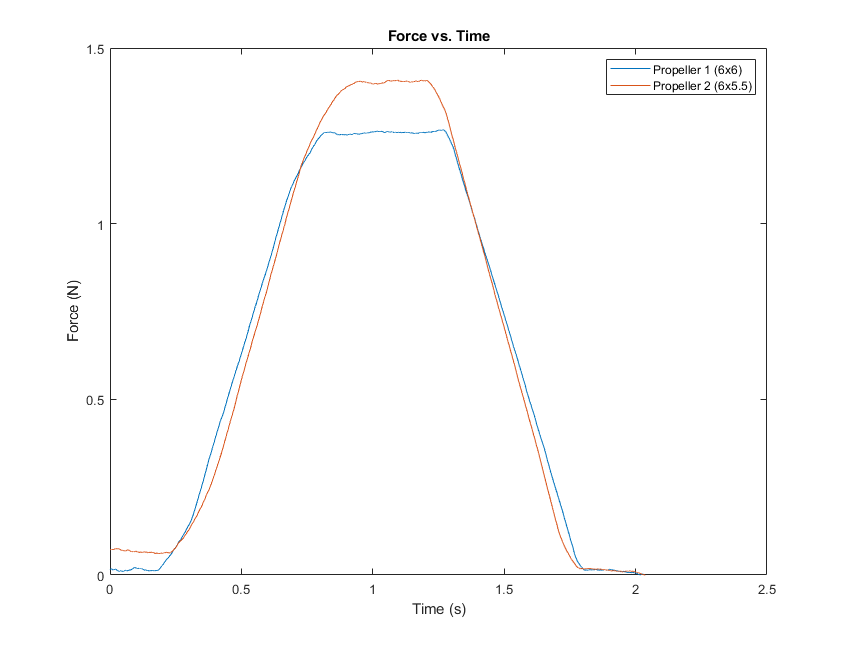
\includegraphics[width = 0.5\textwidth]{finalprojectimages/Trial1_ForcevTime.png}
  \caption{Force vs Time for Trial 1}
  \label{fig:forcevtime}
\end{figure}

\begin{figure}[H]
  \centering
  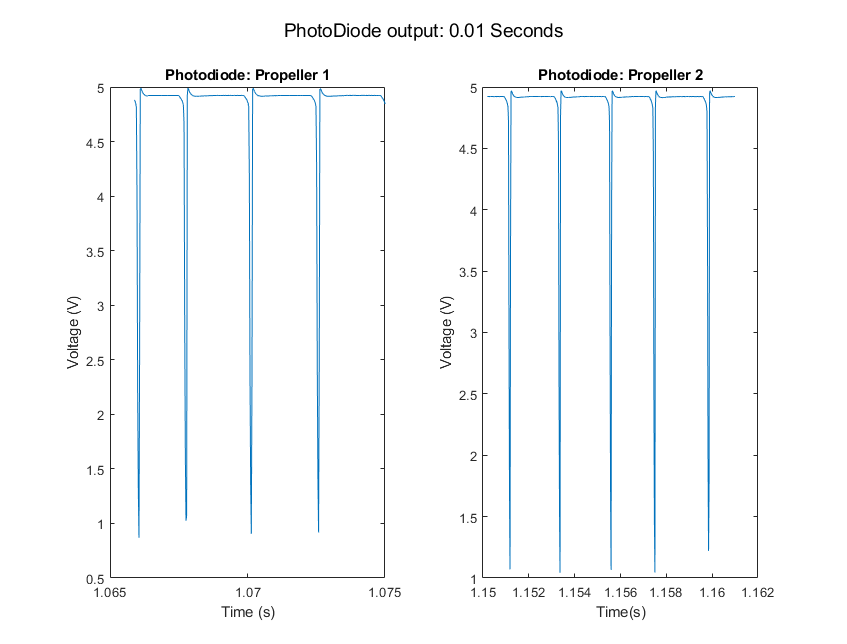
\includegraphics[width = 0.5\textwidth]{finalprojectimages/Trial1_PhotoDiode.png}
  \caption{Photodiode Output for Trial 1}
  \label{fig:photodiode}
\end{figure}

\begin{figure}[H]
  \centering
  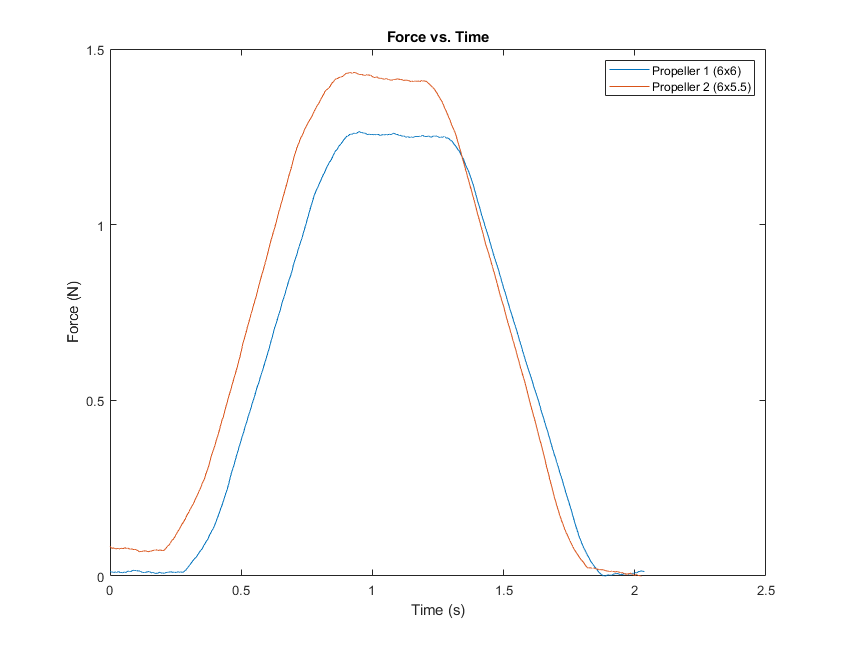
\includegraphics[width = 0.5\textwidth]{finalprojectimages/Trial2_ForcevTime.png}
  \caption{Force vs Time for Trial 2}
  \label{fig:forcevtime2}
\end{figure}

\begin{table}[H]
  \centering
  \begin{tabular}{lcc}
  \hline
  \textbf{Parameter} & \textbf{Propeller 1 (6 x 6)} & \textbf{Propeller 2 (6 x 5.5)} \\
  \hline
  Name & 6 x 6 & 6 x 5.5 \\
  RPM (measured) & 26453.2969 & 27705.3444 \\
  RPM (Theoretical) & 26197 & 26990 \\
  RPM (\% error) & 0.97834 & 2.6504 \\
  Force (N) & 1.2674 & 1.4088 \\
  Wattage (W) & 45.55 & 46.7 \\
  Efficiency & 2.7823 & 3.0168 \\
  Uncertainty (\%) & 0.017541 & 0.016756 \\
  \hline
  \end{tabular}
  \caption{Comparison of Propeller Performance - Trial 1}
  \label{table:propeller_comparison1}
  \end{table}

\begin{table}[h!]
  \centering
  \begin{tabular}{lcc}
  \hline
  \textbf{Parameter} & \textbf{Propeller 1 (6 x 6)} & \textbf{Propeller 2 (6 x 5.5)} \\
  \hline
  Name & 6 x 6 & 6 x 5.5 \\
  RPM (measured) & 25883.3191 & 26272.3077 \\
  RPM (Theoretical) & 26197 & 26990 \\
  RPM (\% error) & 1.1974 & 2.6591 \\
  Force (N) & 1.2653 & 1.4337 \\
  Wattage (W) & 44.25 & 47.3 \\
  Efficiency & 2.8594 & 3.031 \\
  Uncertainty (\%) & 0.017554 & 0.01674 \\
  \hline
  \end{tabular}
  \caption{Comparison of Propeller Performance - Trial 2}
  \label{table:propeller_performance2}
  \end{table}
  

\section{Conclusion}

\newpage
\thispagestyle{empty}  % Clear header/footer
\begin{center}
	\vspace*{\fill}
	{\Huge Appendix}
	\vspace*{\fill}
\end{center}

% Start appendices
\newpage
\begin{appendices}
\pagestyle{fancy}
\renewcommand{\thefigure}{A\arabic{figure}}
\setcounter{figure}{0}

\pagebreak

\hypertarget{datasheets}{}
\section{Datasheets}
\begin{enumerate}[label = {[\arabic*]}]
\small
\item \hypertarget{1}{Multistar Elite 2300KV Motors}
\item ESC
\item Propeller
\item Servo Tester
\item Photodiode
\item NI9215
\item AD623


\end{enumerate}

\end{appendices}

\end{document}
